\atsptt
    \begin{frame}{\ft{Testing the Data Set Application}}
\section{Group 1: Testing the Data Set Application}

        \begin{annotatedFigure}{1pt}{1pt}
            {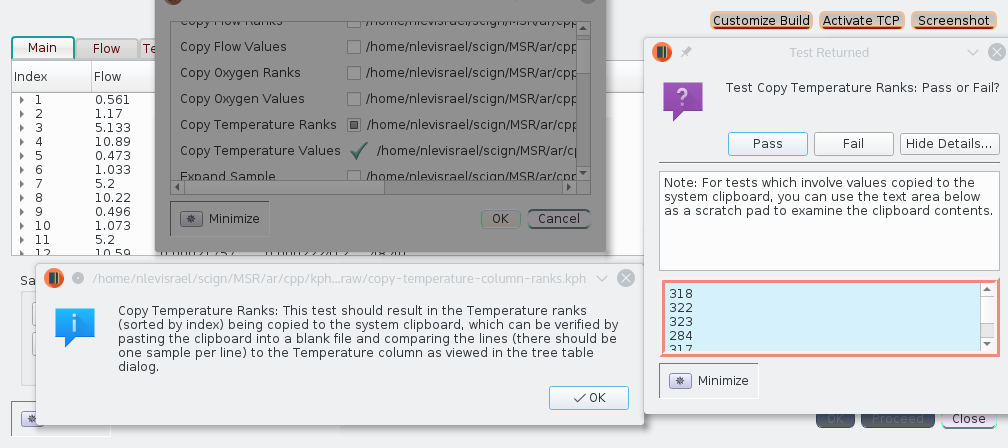
\includegraphics[scale=1.15]{texs/testing.png}}
            
  \node [text width=22cm,inner sep=14pt,align=justify,fill=logoCyan!20, draw=logoBlue, 
  draw opacity=0.5,line width=1mm, fill opacity=0.9]
   at (0.48,1.07){\annfont\textbf{Dataset Creator includes a sophisticated 
   framework for building and running test suites to 
   ensure that raw data is processed correctly and that 
   User Interface components work properly on different 
   Operating System platforms.  This includes 
   a separate testing application that sends instructions 
   to the main Dataset Application via TCP (\circled{1}).}};

  \annotatedFigureBox{0.81,0.93}{0.903,0.982}{1}{0.903,0.935}%
  
  
   \node [text width=4cm,inner sep=14pt,align=justify,fill=logoCyan!20, draw=logoBlue, 
   draw opacity=0.5,line width=1mm, fill opacity=0.9]
    at (0.08,0.64){\annfont\textbf{The testing application has several 
    features to facilitate running tests, including 
    options to repeat tests, mark success or failure (\circled{2}), and 
    examine the system clipboard (\circled{3}).}};
 
  \annotatedFigureBox{0.17,0.63}{0.37,0.685}{2}{0.37,0.63}
   \annotatedFigureBox{0.651,0.113}{0.995,0.86}{3}{0.892,0.86}% 

   \node [text width=11cm,align=justify,fill=logoCyan!20, draw=logoBlue, 
   draw opacity=0.5,line width=1mm, fill opacity=0.9]
    at (0.35,0.125){\textbf{Testers can 
    also read a description of each test (\circled{4}),  
    and view the scripts used to create them.}};
 
  \annotatedFigureBox{0.05,0.16}{0.62,0.325}{4}{0.62,0.19}
  
      %      \annotatedFigureBox{0.222,0.284}{0.3743,0.4934}{B}{0.3743,0.4934}%tr
      %      \annotatedFigureBox{0.555,0.784}{0.6815,0.874}{C}{0.555,0.784}%bl
      %      \annotatedFigureBox{0.557,0.322}{0.8985,0.5269}{D}{0.8985,0.5269}%tr
  
        \end{annotatedFigure}

    \end{frame}


